\section{Dự đoán, đánh giá mô hình và phân tích phần dư}

\subsection{Đường hồi quy tối ưu và Các chỉ số đánh giá}
Đường thẳng hồi quy tối ưu thu được là $ \hat{y} = 12.31 + 0.83x $. Hiệu năng của mô hình trên tập kiểm tra được đánh giá qua các chỉ số:
\begin{itemize}
    \item \textbf{Sai số toàn phương trung bình (MSE):} $31.35$ ms$^2$
    \item \textbf{Hệ số xác định ($R^2$ Score):} $\approx 2.1\%$
\end{itemize}

\textbf{Nhấn mạnh hiệu năng mô hình:} 
Con số $R^2 = 2.1\%$ thoạt nhìn khá khiêm tốn. \textbf{Tuy nhiên, đây không phải là lỗi do thuật toán}. Thuật toán đã tối ưu thành công hàm Loss về sát nghiệm toán học. Con số $2.1\%$ này phản ánh \textbf{thực trạng khách quan của mạng lưới}: Mạng nội bộ (Gateway) không thể giải thích sự biến thiên của tổng độ trễ quốc tế. Lên đến $97.9\%$ sai số hoàn toàn đến từ ngẫu nhiên bên ngoài môi trường mạng.

\subsection{Phân tích phần dư (Residual Analysis)}
\begin{figure}[H]
    \centering
    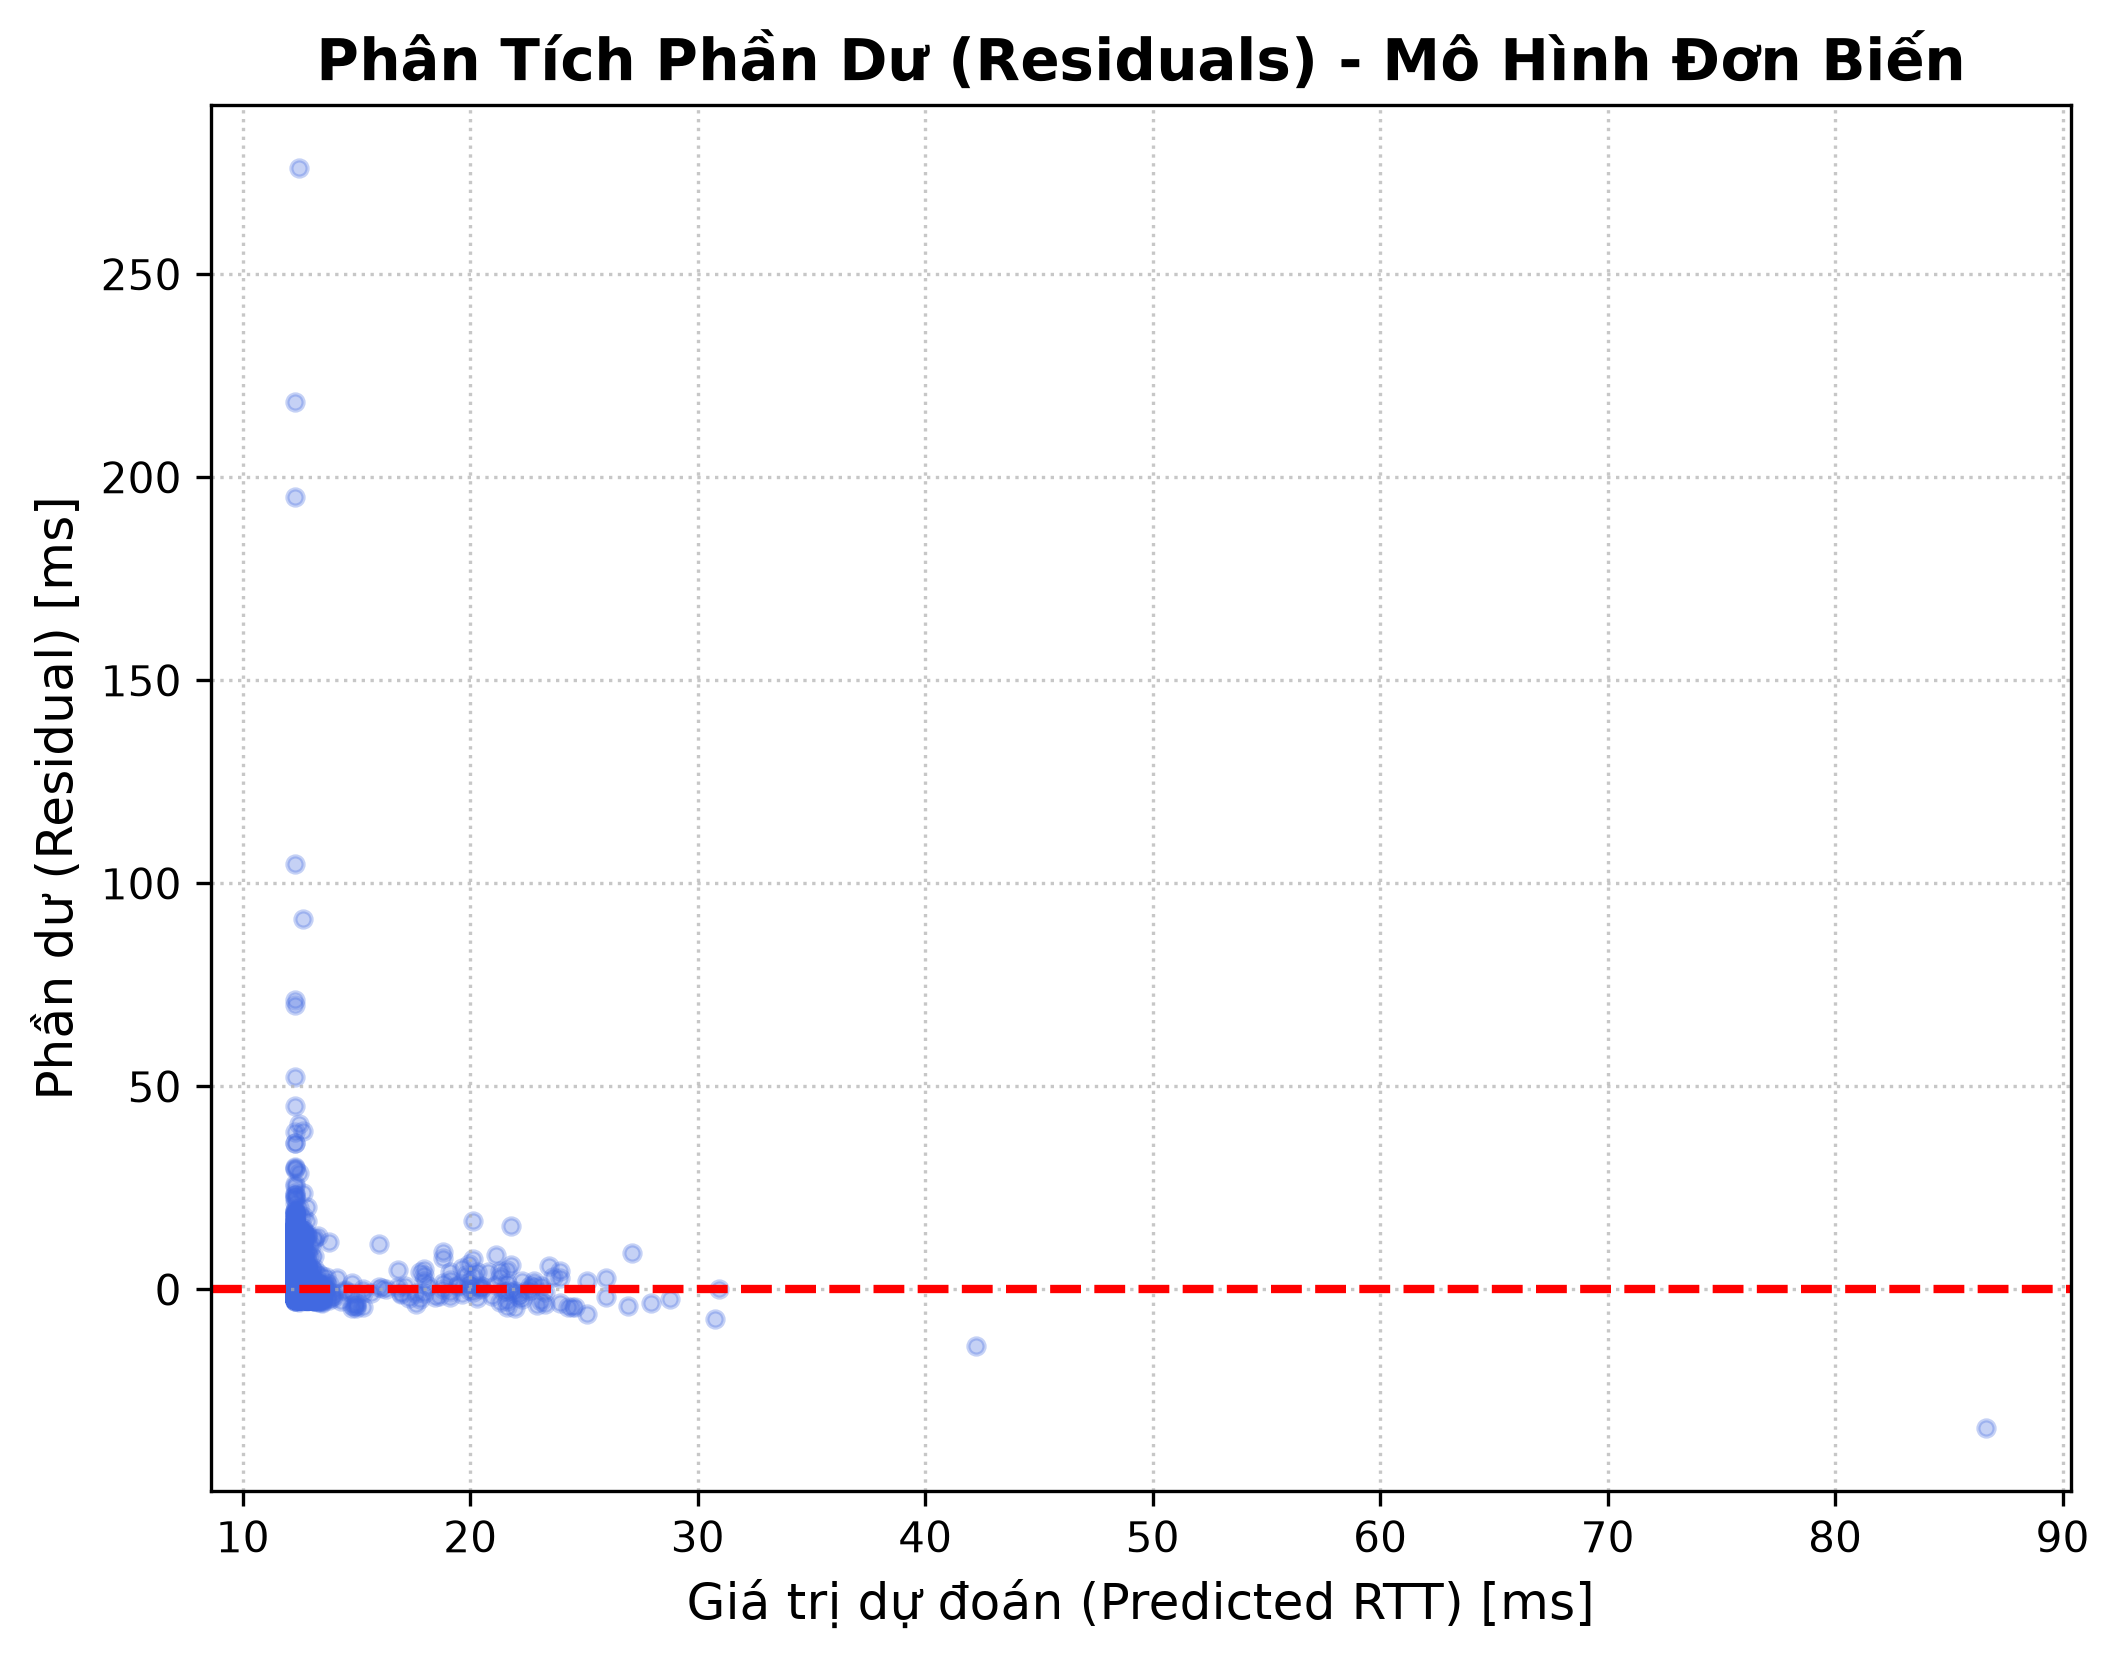
\includegraphics[width=0.8\textwidth]{figures/residual_plot.png}
    \caption{Biểu đồ phần dư theo giá trị dự đoán RTT}
\end{figure}

Đồ thị sơ đồ phần dư cho thấy các sai số xuất hiện \textbf{một vệt thẳng đứng khổng lồ} tại mức dự đoán $\hat{y} \approx 12.3$ ms. Đây là những gói tin có tốc độ ở nhà hoàn hảo, nhưng ra quốc tế bị nghẽn dẫn đến phần dư dương vọt lên tới $300$ ms. Điều này củng cố việc sử dụng mô hình đa biến (Multivariate) ở các phần tiếp theo để dự đoán chính xác hơn.
